\section{Résultats}

\paragraph{Oscillations libres}
Le coefficient d'amortissement et la pulsation du disque ont été déterminé pour des amortissements et masses différentes. Le disque a été laché avec un angle initial de 135°. Conformement à l'\autoref{eq:oscil_libre}, une régression exponentielle sur l'enveloppe du signal a été réalisée afin d'obtenir le coefficient d'amortissement \(\lambda\). Un des signaux obtenus lors de l'expérience est présenté en \autoref{fig:signal_libre}. Le coefficient \(\lambda\) a été déterminé pour 0, 2, ou 3 masses supplémentaires ainsi que pour un amortissment variant entre 0 et 100\%. Les résultats obtenus sont présentés en \autoref{fig:lambda_libre}. Le calcul de la periode \(T\) a été réalisée en prenant une moyenne sur plusieurs periodes, en fonction du nombre de periodes disponnibles, permettant d'obtenir \(\omega = 2 \pi / T\). Cela résulte en une plus grande incertitude sur \(\omega\) pour des grands amortissement. Les détails sur l'estimation des incertitudes sont disponnibles en \autoref{sec:erreurs}. La \autoref{fig:omega_libre} présente les résultats obtenus.

\begin{figure}[h]
    \centering
    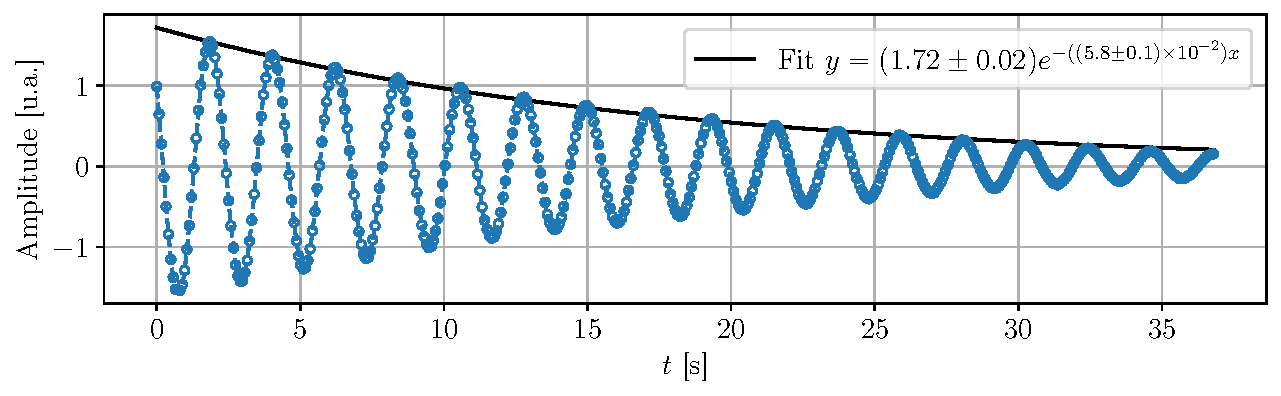
\includegraphics[width=0.9\linewidth]{figures/I3_50_nomot_fitted.pdf}
    \caption{Oscillation libre du disque avec 3 masses supplémentaires et un amortissement de 50\%}
    \label{fig:signal_libre}
\end{figure}

\begin{figure}[h]
    \centering
    \begin{subfigure}{0.48\linewidth}
        \centering
        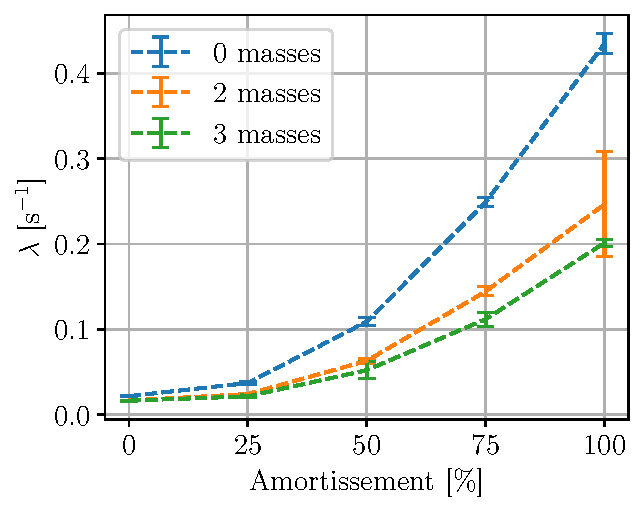
\includegraphics[width=\linewidth]{figures/lambda_nomot.pdf}
        \caption{}
        \label{fig:lambda_libre}
    \end{subfigure}
    \begin{subfigure}{0.48\linewidth}
        \centering
        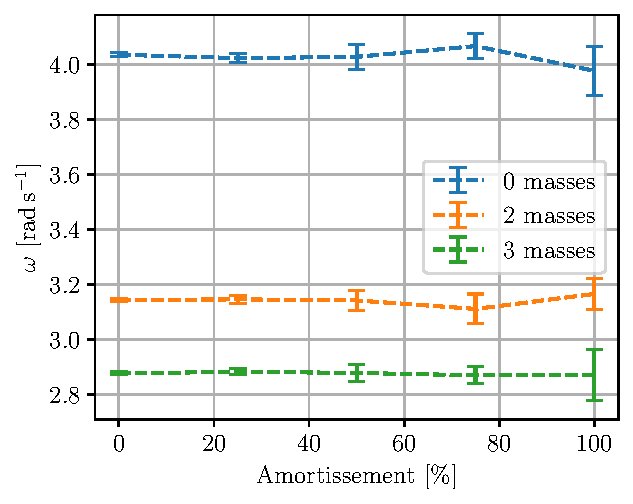
\includegraphics[width=\linewidth]{figures/omega_nomot.pdf}
        \caption{}
        \label{fig:omega_libre}
    \end{subfigure}
    \caption{(a) Le coefficient d'amortissement \(\lambda\) et (b) la pulsation \(\omega\) pour différentes configurations de masses supplémentaires, en fonction de l'amortissement appliqué}
\end{figure}

La pulsation \(\omega_0\) de l'oscillateur harmonique libre sans frottements peut alors être détérminé à partir de l'\autoref{eq:omega_0}. La \autoref{fig:omega0_libre} a été obtenue.

\begin{figure}[h]
    \centering
    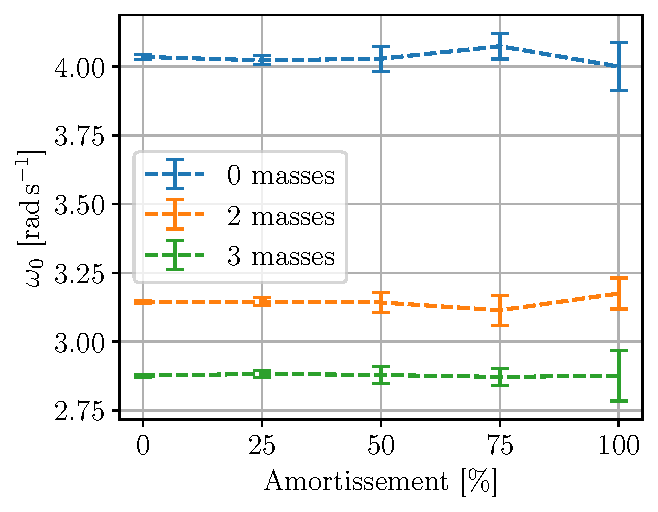
\includegraphics[width=0.5\linewidth]{figures/omega0_nomot.pdf}
    \caption{Pulsation de l'oscillateur harmonique sans frottements en fonction de la configuration}
    \label{fig:omega0_libre}
\end{figure}